\subsection{Interplay of direct and indirect \cp\ violation}
\label{sec:charm:cpvdir}

In decays of $D^0$ mesons, \cp\ asymmetry measurements have contributions from 
both direct and indirect \cp\ violation as discussed in Sec.~\ref{sec:charm:mixcpv}.
The contribution from indirect \cp\ violation depends on the decay-time distribution 
of the data sample~\cite{Kagan:2009gb}. This section describes a combination of 
measurements that allows the extraction of the individual contributions of the 
two types of \cp\ violation.
At the same time, the level of agreement for a no-\cp-violation hypothesis is 
tested. The observables are: 
\begin{equation}
A_{\Gamma} \equiv \frac{\tau(\dbar \ra h^+ h^-) - \tau(D^0 \ra h^+ h^- )}
{\tau(\dbar \ra h^+ h^-) + \tau(D^0 \ra h^+ h^- )},
\end{equation}
where $h^+ h^-$ can be $K^+ K^-$ or $\pi^+\pi^-$, and 
\begin{equation}
\Delta A_{\rm CP}   \equiv A_{\rm CP}(K^+K^-) - A_{\rm CP}(\pi^+\pi^-),
\end{equation}
where $A_{\rm CP}$ are time-integrated \cp\ asymmetries. The underlying 
theoretical parameters are: 
\begin{eqnarray}
a_{\rm CP}^{\rm dir} & \equiv & \frac{|A_{D^0\ra f} |^2 - |A_{\dbar\ra f} |^2} 
{|A_{D^0\ra f} |^2 + |A_{\dbar\ra f} |^2} ,\nonumber\\ 
a_{\rm CP}^{\rm ind}  & \equiv & \frac{1}{2} 
\left[ \left(\left|\frac{q}{p}\right| + \left|\frac{p}{q}\right|\right) x \sin \phi - 
\left(\left|\frac{q}{p}\right| - \left|\frac{p}{q}\right|\right) y \cos \phi \right] ,
\end{eqnarray}
where $A_{D\ra f}$ is the amplitude for $D\ra f$~\cite{Grossman:2006jg}. 
We use the following relations 
between the observables and the underlying parameters~\cite{Gersabeck:2011xj}: 
\begin{eqnarray}
A_{\Gamma} & = & - a_{\rm CP}^{\rm ind} - a_{\rm CP}^{\rm dir} y_{\rm CP},\nonumber\\ 
\Delta A_{\rm CP} & = &  \Delta a_{\rm CP}^{\rm dir} \left(1 + y_{\rm CP} 
\frac{\overline{\langle t\rangle}}{\tau} \right)   +   
   a_{\rm CP}^{\rm ind} \frac{\Delta\langle t\rangle}{\tau}   +   
  a_{\rm CP}^{\rm dir} y_{\rm CP} \frac{\Delta\langle t\rangle}{\tau},\\ 
& \approx & \Delta a_{\rm CP}^{\rm dir} \left(1 + y_{\rm CP} 
\frac{\overline{\langle t\rangle}}{\tau} \right)   +   a_{\rm CP}^{\rm ind} 
\frac{\Delta\langle t\rangle}{\tau}.
\end{eqnarray}
The first relation constrains mostly indirect \cp\ violation, and the 
direct \cp\ violation contribution can differ for different final states. 
In the second relation, $\langle t\rangle/\tau$ denotes the mean decay 
time in units of the $D^0$ lifetime; $\Delta X$ denotes the difference 
in quantity $X$ between $K^+K^-$ and $\pi^+\pi^-$ final states; and $\overline{X}$ 
denotes the average for quantity $X$. 
We neglect the last term in this relation as all three factors are 
$\mathcal{O}(10^{-2})$ or smaller, and thus this term is negligible 
with respect to the other two terms. 
Note that $\Delta\langle t\rangle/\tau \ll\langle t\rangle/\tau$, and 
it is expected that $|a_{\rm CP}^{\rm dir}| < |\Delta a_{\rm CP}^{\rm dir}|$ 
because $a_{\rm CP}^{\rm dir}(K^+K^-)$ and $a_{\rm CP}^{\rm dir}(\pi^+\pi^-)$ 
are expected to have opposite signs. 

In this fit, $A_\Gamma(KK)$ and $A_\Gamma(\pi\pi)$ are assumed to be identical.
This assumption is supported by the most recent LHCb measurements~\cite{Aaij:2013ria}.
A significant relative shift due to final-state dependent $A_\Gamma$ values between $\Delta A_{\rm CP}$ measurements with different mean decay times is excluded by these measurements.

A $\chi^2$ fit is performed in the plane $\Delta a_{\rm CP}^{\rm dir}$ 
vs. $a_{\rm CP}^{\rm ind}$. 
For the \babar result the difference of the quoted values for 
$A_{\rm CP}(K^+K^-)$ and $A_{\rm CP}(\pi^+\pi^-)$ is calculated, 
adding all uncertainties in quadrature. 
This may overestimate the systematic uncertainty for the difference 
as it neglects correlated errors; however, the result is conservative 
and the effect is small as all measurements are statistically limited. 
For all measurements, statistical and systematic uncertainties are added 
in quadrature when calculating the $\chi^2$. 
We use the current world average value $y_{\rm CP} = (0.866 \pm 0.155)\%$ 
(see Sec.~\ref{sec:charm:mixcpv}) and the measurements listed in 
Table~\ref{tab:charm:dir_indir_comb}. 

\begin{table}
\centering 
\caption{Inputs to the fit for direct and indirect \cp\ violation. 
The first uncertainty listed is statistical, and the second is systematic.}
\label{tab:charm:dir_indir_comb}
\vspace{3pt}
\begin{tabular}{ll|ccccc}
\hline \hline
Year & 	Experiment	& Results
& $\Delta \langle t\rangle/\tau$ & $\langle t\rangle/\tau$ & Reference\\
\hline
2012	& Belle	prel. & $A_\Gamma = (-0.03 \pm 0.20 \pm 0.08 )\%$ &	-&	-&	 
\cite{Staric:2012ta}\\
2012	& \babar	& $A_\Gamma = (0.09 \pm 0.26 \pm 0.06 )\%$ &	-&	-&	 
\cite{Lees:2012qh}\\
2013	& LHCb	& $A_\Gamma(KK) = (-0.035 \pm 0.062 \pm 0.012 )\%$ &	-&	-&	 
\cite{Aaij:2013ria}\\
    	&     	& $A_\Gamma(\pi\pi) = (0.033 \pm 0.106 \pm 0.014 )\%$ &	-&	-&	 
                   \\
2008	& \babar	& $A_{\rm CP}(KK) = (0.00 \pm 0.34 \pm 0.13 )\%$&&&\\ 
& & $A_{\rm CP}(\pi\pi) = (-0.24 \pm 0.52 \pm 0.22 )\%$ &	$0.00$ &	
$1.00$ &	 \cite{Aubert:2007if}\\
2012	& Belle	prel. & $\Delta A_{\rm CP} = (-0.87 \pm 0.41 \pm 0.06 )\%$ &	
$0.00$ &	$1.00$ &	 \cite{Ko:2012px}\\
2012	& CDF	 & $\Delta A_{\rm CP} = (-0.62 \pm 0.21 \pm 0.10 )\%$ &	
$0.25$ &	$2.58$ &	 \cite{Collaboration:2012qw}\\
2013	& LHCb	prel. & $\Delta A_{\rm CP} = (-0.34 \pm 0.15 \pm 0.10 )\%$ &	
$0.11$ &	$2.10$ &	 \cite{LHCb:2013dka}\\
2014	& LHCb	& $\Delta A_{\rm CP} = (0.14 \pm 0.16 \pm 0.08 )\%$ &	
$0.01$ &	$1.07$ &	 \cite{Aaij:2014gsa}\\
\hline
\end{tabular}
\end{table}

The combination plot shows the measurements listed in 
Table~\ref{tab:charm:dir_indir_comb} for
$\Delta A_{\rm CP}$ and $A_\Gamma$, where the bands represent $\pm1\sigma$ 
intervals.  The point of no \cp\ violation (0,0) is shown as a filled circle, 
and two-dimensional $68\%$ CL, $95\%$ CL, and $99.7\%$ CL regions are plotted 
as ellipses. The best fit value is indicated by a cross showing the
one-dimensional errors.

\begin{figure}
\begin{center}
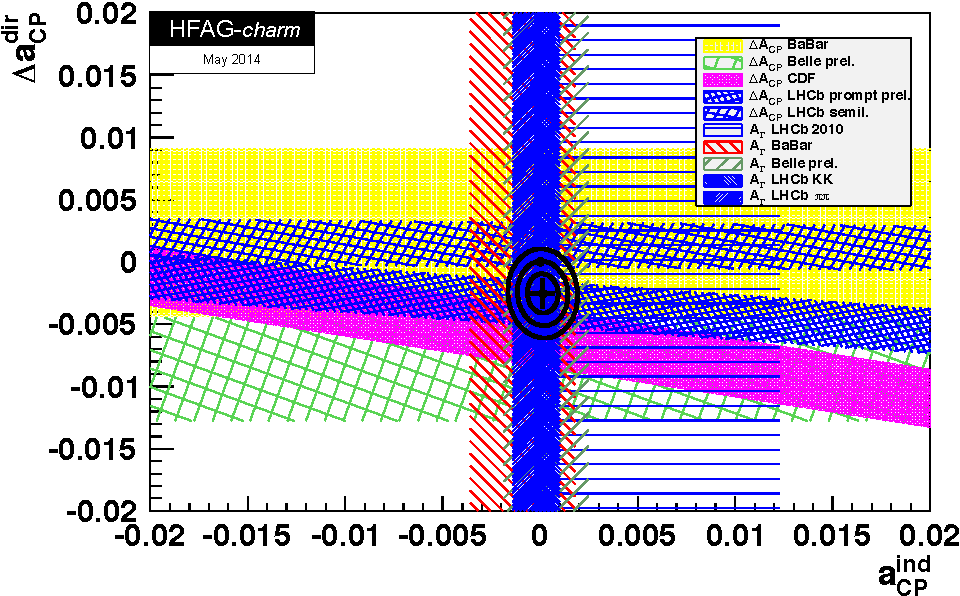
\includegraphics[width=0.90\textwidth]{figures/charm/deltaACP_AGamma_fit_May14.pdf}
\caption{Plot of all data and the fit result. Individual 
measurements are plotted as bands showing their $\pm1\sigma$ range. 
The no-\cpv\ point (0,0) is shown as a filled circle, and the best 
fit value is indicated by a cross showing the one-dimensional errors. 
Two-dimensional $68\%$ CL, $95\%$ CL, and $99.7\%$ CL regions are 
plotted as ellipses. }
\label{fig:charm:dir_indir_comb}
\end{center}
\end{figure}

From the fit, the change in $\chi^2$ from the minimum value for the no-\cpv\ 
point (0,0) is $5.9$, which corresponds to a CL of $5.1\times 10^{-2}$ for 
two degrees of freedom. Thus the data are consistent with the no-\cp-violation 
hypothesis at $5.1\%$ CL. This p-value corresponds to $2.0\sigma$. The central values and $\pm1\sigma$ errors for 
the individual parameters are
\begin{eqnarray}
a_{\rm CP}^{\rm ind} & = & (0.013 \pm 0.052 )\% \nonumber\\
\Delta a_{\rm CP}^{\rm dir} & = & (-0.253 \pm 0.104 )\%.
\end{eqnarray}
These results indicate that the origin of this \cp\ violation lies in the 
difference between direct \cp\ violation in the two final states, rather 
than in a common indirect \cp\ violation.


